\byline{{\textbf{\Large\sffamily November Bonsai Club Meetup:}}\\
{\textbf{\large\sffamily Natural Style, Inspired Learning}}}{The Newsletter Team}
\noindent
After the recent Annual General Meeting (a brief summary of which is available at p.~\pageref{agm-summary}) our members gathered once again for an evening of shared enthusiasm and bonsai inspiration. 
This time, we had the pleasure of welcoming the incredibly talented \textbf{David Cheshire}, well known for his \href{https://www.davidcheshirenurseries.co.uk}{renowned nursery} and for championing a more natural style of bonsai inspired by his travels to Japan.
%
David guided us through the techniques he applies to a wide range of species, including \textbf{Maples}, \textbf{Junipers}, \textbf{Oaks}, and several others. 
What made the evening particularly special was the array of trees he brought with him --- from youthful starters to mature specimens --- each one demonstrating the long\--term results of his methods. 
His talk offered both practical insight and artistic inspiration, giving members plenty to think about for their own collections.
%
It wasn't just our \textbf{23 regular members} who enjoyed the presentation. We were also delighted to be joined by two special guests: \textbf{Mark and Mingchen Moreland} from the \href{https://www.ukbonsaiassoc.org}{UK Bonsai Association}, who came along especially to hear David speak. A more detailed report on his presentation can be found later in this newsletter at p.~\pageref{workshop}.

\medskip
Alongside the talk, we held our monthly \textbf{Tree of the Month} competition. This month's challenge invited both Novice and General members to bring back a tree they had previously shown earlier in the year. The result was a strong and varied display, reflecting real progress and refinement from everyone who took part. More photos and details are included at p.~\pageref{contest}.
%
A warm and delicious \textbf{honourable mention} goes once again to \textbf{Adam} for his fantastic cupcakes, rapidly becoming a much\--anticipated club tradition! Thank you, Adam, and thank you to every member who helped make the evening another memorable success.

\medskip
We look forward to seeing you all again on \textbf{11th December at 7pm} at the \textbf{Whitton Community Centre}, TW2 6JL, for our final meeting of the year themed \emph{``Festive Fun \& Party Time!''}.
\medskip

\vspace*{-1em}
\begin{window}[2,l,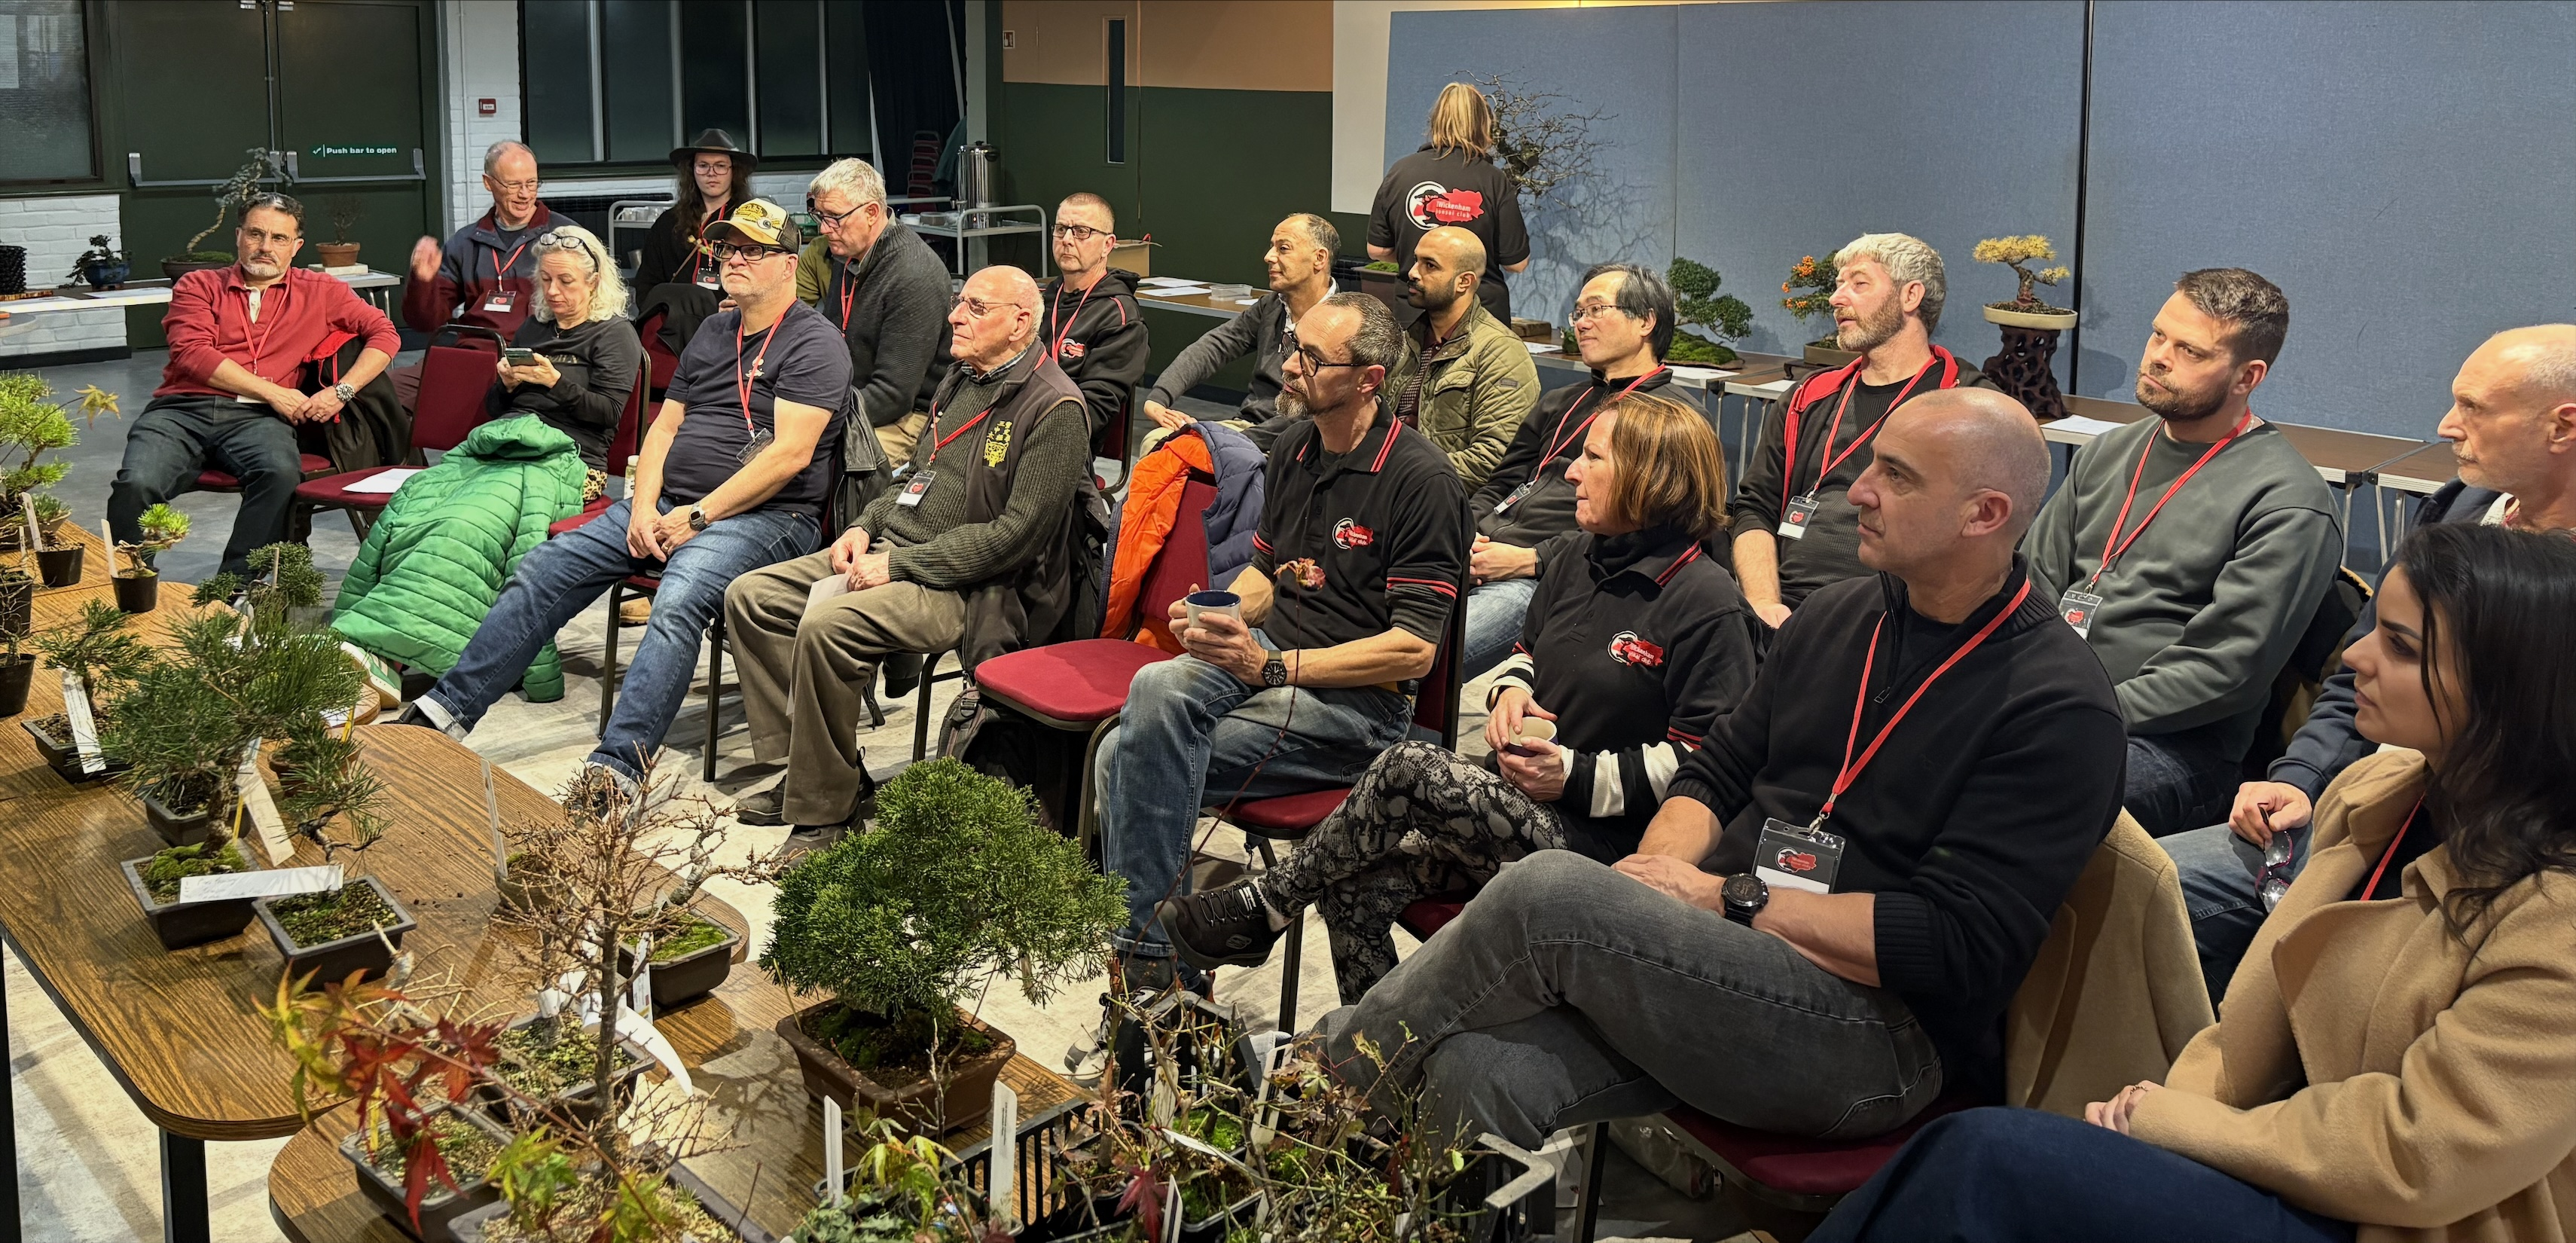
\includegraphics[width=1.0\columnwidth]{2025_11/res/editorial_cheshire.jpg},\centerline{\emph{Regular members and guests attentively listen to David Cheshire's techniques.}}]
\end{window}
\vspace*{-1em}
\closearticle
\clearpage
